\begin{definition}
	\textit{Нормой оператора} $A$ называется инфимум по всем ограничивающим константам:
	\[
		\|A\| := \inf \{K \colon \forall x \in E_1\ \|Ax\| \le K\|x\|\}
	\]
\end{definition}

\begin{proposition} (не по лектору)
	Для нормы оператора $A$ всегда выполнено неравенство:
	\[
		\forall x \in E_1\ \ \|Ax\| \le \|A\| \cdot \|x\|
	\]
	Причём оператор ограничен тогда и только тогда, когда $\|A\| < \infty$.
\end{proposition}

\begin{proof}
	Эквивалентность очевидна. Нужно лишь пояснить, почему в конечном случае для точной нижней грани, коей является $\|A\|$, действительно работает неравенство. Это несложно, ведь точно существует последовательность подходящих сверху констант $\{K_n\}_{n = 1}^\infty$, $\lim_{n \to \infty} K_n = \|A\|$. А тогда мы при каждом отдельном $x \in E_1$ просто используем предельный переход в неравенстве, требуемое доказано.
\end{proof}

\begin{proposition}
	Для нормы оператора $A$ верны равенства:
	\[
		\|A\| = \sup_{\|x\| \le 1} \|Ax\| = \sup_{\|x\| = 1} \|Ax\| = \sup_{x \neq 0} \frac{\|Ax\|}{\|x\|}
	\]
\end{proposition}

\begin{proof}
	Определение ограниченности линейного оператора имеет эквивалентный вид, как мы уже доказали:
	\[
		\exists K \in \K \such \forall y \in S(0, 1)\ \ \|Ay\| \le K
	\]
	По определению, $\|A\|$ --- точная нижняя грань всех подходящих констант. В силу эквивалентного определения должно быть очевидно, что $\sup_{y \in S(0, 1)} \|Ay\|$, во-первых, будет оценивать сверху необходимую норму, а во-вторых, меньше взять не получится уже в силу определения точной верхней грани, то есть равенство определения и второго выражения установлено.
	
	Для установления равенства между первым и вторым выражениями достаточно заметить, что все точки $0 < \|x\| < 1$ являются на самом деле некоторым $\alpha y$, где $\alpha \in (0; 1)$ и $\|y\| = 1$, поэтому $\|Ax\| = |\alpha| \cdot \|Ay\| \le \|Ay\|$, то есть особого смысла точки внутри единичного шара не несут.
	
	Третье выражение вообще получается почти без изменений определения ограниченности. Заметим, что его также можно записать в таком виде:
	\[
		\exists K \in \K \such \forall x \neq 0\ \|Ax\| \le K\|x\| \Lra \frac{\|Ax\|}{\|x\|} \le K
	\]
	Дальше идея та же, что и для второго выражения.
\end{proof}

\begin{note}
	Эти формулы играют очень важную роль при поиске нормы оператора, ибо для этой задачи нет какого-то общего алгоритма. Однако обычно делают так: вначале находят оценку в духе определения ограниченности, а затем, если вера в её неулучшаемость непоколебима, используют одно из супремумных определений. Если значение супремума сошлось к тому, что мы получили ранее, то норма оператора найдена.
\end{note}

\begin{proposition}
	Пусть $A$ --- линейный непрерывный в точке $x_0 \in E_1$ оператор. Тогда $A$ непрерывен.
\end{proposition}

\begin{proof}
	Действительно, рассмотрим произвольную точку $x \in E_1$. Тогда мы хотим доказать следующее утверждение:
	\[
		\forall \{x_n\}_{n = 1}^\infty \subseteq E_1\ \Big(\lim_{n \to \infty} x_n = x \ra \lim_{n \to \infty} Ax_n = Ax\Big)
	\]
	Идея состоит в том, что линейность оператора даёт нам в каком-то смысле параллельный перенос аргумента. Действительно, мы можем сказать следующее:
	\[
		x_0 = x - (x - x_0) = \lim_{n \to \infty} x_n - (x - x_0) \Ra \lim_{n \to \infty} A(x_n - (x - x_0)) = Ax_0
	\]
	Переход к пределу с оператором мы сделали по условию. Осталось просто переставить части выражения, ибо есть линейность:
	\[
		\lim_{n \to \infty} A(x_n - (x - x_0)) = \lim_{n \to \infty} (Ax_n - Ax + Ax_0) = Ax_0 \Ra \lim_{n \to \infty} Ax_n = Ax
	\]
\end{proof}

\begin{theorem}
	Пусть $A \colon E_1 \to E_2$ --- линейный оператор. Тогда $A$ ограничен тогда и только тогда, когда он непрерывен.
\end{theorem}

\begin{proof}~
	\begin{itemize}
		\item[$\Ra$] По условию мы знаем, что
		\[
			\forall x \in E_1\ \ \|Ax\| \le \|A\| \cdot \|x\|
		\]
		С другой стороны, рассмотрим последовательность $\{x_n\}_{n = 1}^\infty \subseteq E_1$, сходящуюся к $x \in E_1$. Тогда:
		\[
			\|Ax_n - Ax\| = \|A(x_n - x)\| \le \|A\| \cdot \|x_n - x\| \xrightarrow[n \to \infty]{} 0
		\]
		
		\item[$\La$] Пойдём от противного. Тогда оператор должен быть и непрерывен, и неограничен. Последнее можно записать так:
		\[
			\forall n \in \N\ \exists x_n \in E_1 \bs \{0\} \such \|Ax_n\| > n\|x_n\|
		\]
		Занесём всю правую часть в аргумент оператора. Тогда:
		\[
			\forall n \in \N\ \exists x_n \in E_1 \bs \{0\} \such \Bigg\|A\underbrace{\frac{x_n}{n\|x_n\|}}_{y_n}\Bigg\| > 1
		\]
		Несложно увидеть, что $\lim_{n \to \infty} \|y_n\| = \lim_{n \to \infty} \frac{1}{n} = 0$, а стало быть $\lim_{n \to \infty} y_n = 0$. Но так как оператор $A$ непрерывен, отсюда мы также получаем предел $\lim_{n \to \infty} Ay_n = A0 = 0$, чья норма противоречит неравенству выше.
	\end{itemize}
\end{proof}

\begin{definition}
	\textit{Множество всех линейных ограниченных операторов} обозначается как $\cL(E_1, E_2)$.
\end{definition}

\begin{note}
	Укажем 2 важных частных случая:
	\begin{itemize}
		\item $\cL(E) := \cL(E, E)$
		
		\item $E^* := \cL(E, \R)$
	\end{itemize}
\end{note}

\begin{theorem}
	Имеет место 2 утверждения:
	\begin{enumerate}
		\item $\cL(E_1, E_2)$ --- нормированное пространство с нормой, порождённой нормой операторов
		
		\item Если $E_2$ --- банахово пространство, то и $\cL(E_1, E_2)$ --- банахово пространство
	\end{enumerate}
\end{theorem}

\begin{proof}~
	\begin{enumerate}
		\item Линейность пространства тривиальна. Для того, чтобы доказать корректность нормы, нам достаточно проверить неравенство треугольника (остальное просто очевидно):
		\[
			\|A_1 + A_2\| = \sup_{\|x\| = 1} \|A_1x + A_2x\| \le \sup_{\|x\| = 1} \|A_1x\| + \sup_{\|x\| = 1} \|A_2x\| = \|A_1\| + \|A_2\|
		\]
		
		\item Нужно показать полноту пространства. Пусть $\{A_n\}_{n = 1}^\infty \subseteq \cL(E_1, E_2)$ --- фундаментальная последовательность:
		\[
			\forall \eps > 0\ \exists N \in \N \such \forall n, m \ge N\ \ \|A_n - A_m\| < \eps
		\]
		Покажем, что есть поточечная сходимость. Действительно:
		\[
			\forall x \in E_1\ \ \|A_nx - A_mx\| \le \|A_n - A_m\| \cdot \|x\| < \eps \|x\|
		\]
		Стало быть, последовательность $\{A_nx\}_{n = 1}^\infty \subseteq E_2$ фундаментальна при любом фиксированном $x \in E_1$, а в силу банаховости $E_2$ сходится. Определим оператор $A$ следующим образом:
		\[
			\forall x \in E_1\ \ Ax := \lim_{n \to \infty} A_nx
		\]
		Осталось показать, что этот оператор удовлетворяет всем требованиям:
		\begin{itemize}
			\item $A$ линеен. Здесь мы просто воспользуемся свойствами пределов:
			\begin{multline*}
				\forall x, y \in E_1, \alpha, \beta \in \K\ \ A(\alpha x + \beta y) = \lim_{n \to \infty} A_n(\alpha x + \beta y) =
				\\
				\alpha \lim_{n \to \infty} A_nx + \beta \lim_{n \to \infty} A_ny = \alpha Ax + \beta Ay
			\end{multline*}
			
			\item $A$ ограничен. Мы уже знаем в силу определения этого оператора, что \\ $\lim_{n \to \infty} \|A_nx\| = \|Ax\|$, причём $\|A_nx\| \le \|A_n\| \cdot \|x\|$. Если бы у всех норм операторов была общая оценка сверху, то по предельному неравенству мы бы получили оценку и для $A$. В самом деле, последовательность $\{A_n\}_{n = 1}^\infty$ фундаментальна, а стало быть ограничена.
			
			\item Верно, что $\lim_{n \to \infty} A_n = A$. По определению мы должны показать предел \\ $\lim_{n \to \infty} \|A_n - A\| = 0$. Это можно сделать так: зафиксируем $\eps > 0$ и рассмотрим произвольный $x \in E_1$. За счёт фундаментальности $\{A_n\}_{n = 1}^\infty$:
			\[
				\forall \eps > 0\ \exists N \in \N \such \forall x \in E_1\  \forall m > n \ge N\ \ \|A_nx - A_mx\| \le \|A_n - A_m\| \cdot \|x\| < \eps\|x\|
			\]
			Устремим $m$ в бесконечность. Так можно сделать, в силу существования этого предела:
			\[
				\forall \eps > 0\ \exists N \in \N \such \forall x \in E_1\ \forall n \ge N\ \ \|A_nx - Ax\| < \eps \|x\|
			\]
			В силу линейности, можно переписать это утверждение, рассматривая только единичную сферу:
			\[
				\forall \eps > 0\ \exists N \in \N \such \forall x \in S(0, 1)\ \forall n \ge N\ \ \|A_nx - Ax\| < \eps
			\]
			Итак, осталось воспользоваться эквивалентным определением нормы оператора:
			\[
				\forall \eps > 0\ \exists N \in \N \such \forall n \ge N\ \ \|A_n - A\| = \sup_{\|x\| = 1} \|A_nx - Ax\| < \eps
			\]
		\end{itemize}
	\end{enumerate}
\end{proof}

\begin{corollary}~
	\begin{itemize}
		\item Если $E$ --- банахово пространство, то и $\cL(E)$ банахово.
		
		\item Для любого линейного нормированного пространства $E$ верно, что $E^*$ --- банахово пространство
	\end{itemize}
\end{corollary}

\begin{example}
	Существует ли оператор, который был бы линейным, но не ограниченным?
	
	Оказывается, что в конечномерном случае нет, а в бесконечномерном --- да. Рассмотрим $E_1 = C^1[0; 1]$ с нормой $C[0; 1]$, $E_2 = C[0; 1]$ и пространство $\cL(E_1, E_2)$. Оператор дифференцирования $\frac{d}{dx}$ является линейным, но при этом неограничен (это то же самое, что и не непрерывен):
	\[
		\frac{\sin(nx)}{n} \rra 0;\ \ \frac{d}{dx} \frac{\sin(nx)}{n} = \cos(nx) \centernot\rra \frac{d}{dx} 0 = 0
	\]
\end{example}

\begin{theorem} (о продолжении линейного ограниченного оператора) \label{op_cont_th}
	Пусть $D(A) \subseteq E_1$ --- линейное многообразие, причём $\cl D(A) = E_1$ Тогда для любого линейного ограниченного оператора $A \colon D(A) \to E_2$ существует согласованный оператор $\tilde{A} \in \cL(E_1, E_2)$ такой, что
	\begin{enumerate}
		\item $\tilde{A}|_{D(A)} = A$
		
		\item $\|\tilde{A}\| = \|A\|$
	\end{enumerate}
\end{theorem}

\begin{theorem} (1927г. Банаха-Штейнгауза-Хана, принцип равномерной ограниченности)
	Пусть $E_1$ --- банахово пространство, $\{A_n\}_{n = 1}^\infty \subseteq \cL(E_1, E_2)$. Тогда верна импликация:
	\[
		\Big(\forall x \in E\ \ \sup_{n \in \N} \|A_n x\| < \infty\Big) \Ra \sup_{n \in \N} \|A_n\| < \infty
	\]
\end{theorem}

\begin{proof}
	Запишем утверждение теоремы в эквивалентной форме:
	\[
		\sup_{n \in \N} \|A_n\| = \infty \Ra \Big(\exists x \in E_1 \such \sup_{n \in \N} \|A_nx\| = \infty\Big)
	\]
	Именно в такой форме мы и докажем требуемое. Далее мы считаем, что $\sup_{n \in \N} \|A_n\| = \infty$. Проведём доказательство в 2 шага (основная идея схожа с теоремой Бэра, и даже есть доказательства, которые на неё прямо опираются, но мы пойдём другой дорогой):
	\begin{enumerate}
		\item Покажем, что если последовательность операторов $\{A_n\}_{n = 1}^\infty$ равномерно ограничена хотя бы на каком-то замкнутом шаре $\ole{B}(x_0, r)$, то уже $\sup_{n \in \N} \|A_n\| < \infty$. Действительно, это утверждение можно записать так:
		\[
			\exists M > 0 \such \forall x \in \ole{B}(x_0, r), n \in \N\ \ \|A_nx\| \le M
		\]
		
		Идея состоит в том, что у этого замкнутого шара для любой точки $x \in E_1$ есть соответствующий радиус-вектор $y - x_0$, который сонаправлен $x$.
		
		\begin{center}
			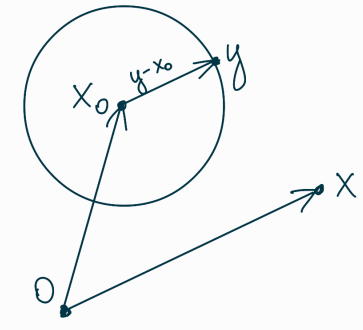
\includegraphics[width=0.3\textwidth]{images/3pic.png}
		\end{center}
		
		Их связь можно записать так:
		\[
			r \cdot \frac{x}{\|x\|} = y - x_0 \Ra x = \frac{\|x\|}{r}(y - x_0)
		\]
		Через линейность получаем оценку нормы $A_nx$:
		\[
			\forall n \in \N\ \ \|A_nx\| = \frac{\|x\|}{r}\|A_ny - A_nx_0\| \le \frac{2M}{r}\|x\|
		\]
		Что и требовалось.
		
		\item В силу доказанного и имеющегося предположения, у нас нет ни одного замкнутого шара, где последовательность операторов была бы равномерно ограничена. В силу банаховости $E_1$, мы получим искомую точку $x$ через последовательность вложенных замкнутых шаров. Возьмём произвольный $\ole{B_0}(x_0, 1)$ и рассмотрим также $\ole{B_0}(x_0, 1 / 2)$ В силу уже сказанного, найдётся точка $x_1$:
		\[
			\exists x_1 \in \ole{B}_0(x_0, 1 / 2), n_1 \in \N \such \|A_{n_1}x_1\| > 1
		\]
		Коль скоро оператор $A_{n_1}$ непрерывен, мы найдём некоторый шарик $\ole{B}_1(x_1, r_1)$, $r_1 < 1 / 2$, в котором любая точка также будет удовлетворять неравенству. В шаре \\ $\ole{B}_1(x_1, r_1 / 2)$ аналогично ищем $x_2$ и $n_2 > n_1$ такие, чтобы выполнилось неравенство $\|A_{n_2}x_2\| > 2$. Продолжая алгоритмические действия счётное число раз, мы получим последовательность вложенных вложенных шаров $\ole{B}_k(x_k, r_k)$, чьи радиусы тривиально стремятся к нулю (если говорить строго, то верно соотношение $r_k < r_{k - 1} / 2$), причём верно утверждение:
		\[
			\forall x \in \ole{B}_k(x_k, r_k)\ \ \|A_{n_k}x\| > k
		\]
		В силу полноты пространства $E_1$, верна теорема о вложенных шарах и, следовательно, есть точка в пересечении:
		\[
			\exists x = \lim_{k \to \infty} x_k \in \bigcap_{k = 1}^\infty \ole{B}_k(x_k, r_k) \Lora \forall k \in \N\ \ \|A_{n_k}x\| > k \Ra \sup_{n \in \N} \|A_nx\| = \sup_{k \in \N} \|A_{n_k}x\| = \infty
		\]
	\end{enumerate}
\end{proof}

\begin{anote}
	По сути теорема Банаха-Штейнгауза-Хана говорит нам, что при наличии поточечной ограниченности (то есть $A_nx$ не убегает куда-то в бесконечность с ростом $n$), у нас имеется ограниченность последовательности операторов $\{A_n\}_{n = 1}^\infty$. Этот важный факт позволяет доказать полноту $\cL(E_1, E_2)$ относительно поточечной сходимости.
\end{anote}
